\subsection[Full NLO calculation with free MH and mt]{Full NLO calculation with free \boldmath $m_h$ and $m_t$}
\label{sec:nlo2}

%\textit{Authors:} J. Baglio, F. Campanario, S. Glaus, M. M. M\"uhlleitner, J. Ronca, M. Spira, J. Streicher (2003.03227 + 1811.05692) \\[0.3cm]

\textbf{Julien Baglio, Francisco Campanario, Seraina Glaus, Milada Margarete Mühl\-leitner, Jonathan Ronca, Michael Spira, Juraj Streicher~\cite{Baglio:2018lrj,Baglio:2020ini}.}

\begin{figure}[!hbtp]
\vspace*{-0cm}
\begin{center}
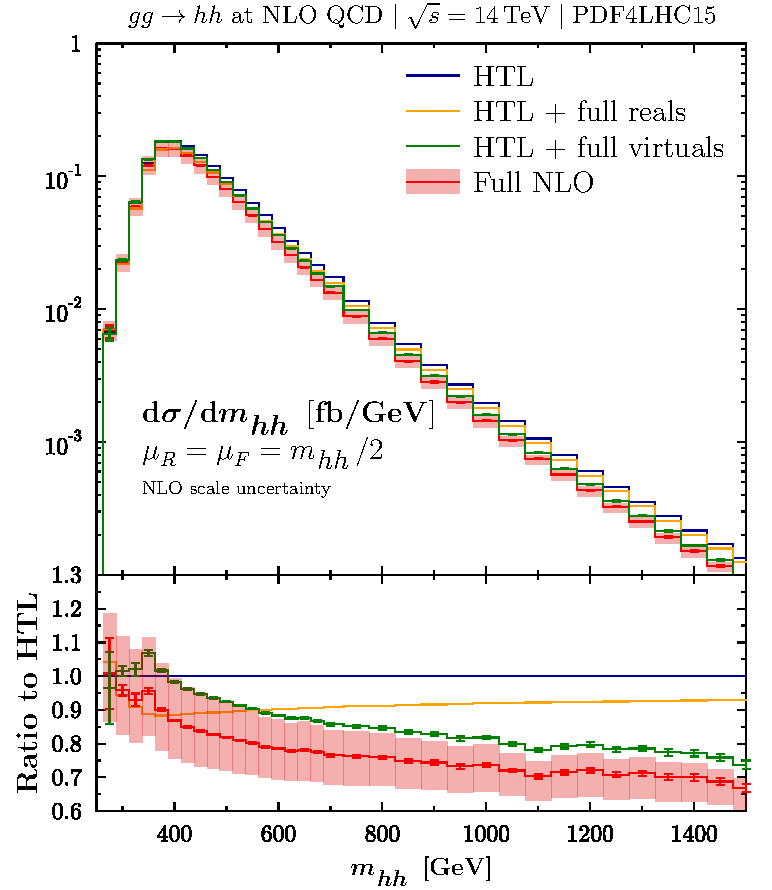
\includegraphics[width=0.5\textwidth]{NLO_QCD_SM/NLOmtmh/Images/hh_nlo_pdf4lhc_14tev_mhh_title_fixed.pdf}
\vspace*{-0cm}
\caption{Invariant-mass distributions for Higgs boson pair production via gluon fusion at the 14 TeV LHC as a function of $m_{hh}$. LO results (in black), HTL results (in blue), HTL results including the full real corrections (in yellow), HTL results including the full virtual corrections (in green, including the numerical error), and the full NLO QCD results (in red, including the numerical error). Results shown are from Refs.~\cite{Baglio:2018lrj,Baglio:2020ini}.}
\label{fg:dist_mhh}
\end{center}
\end{figure}
\noindent A second independent numerical calculation of the NLO QCD corrections, including the full top quark mass dependence, has been performed in Refs.~\cite{Baglio:2018lrj,Baglio:2020ini,Baglio:2020wgt}. In these works, the projection onto the two contributing form factors has been utilized in $D$ dimensions, with Feynman parametrization applied diagram by diagram, with no tensor reduction. This leads to compact expressions such that the free choice of Higgs boson and top quark masses could be retained. Since the bottom loops contribute at the percent level only, they have been neglected. The singularities were isolated by suitable end-point subtractions and dedicated infrared subtraction terms that built on the explicit structure of the Feynman-parameter integrals. The virtual $t\bar t$ thresholds were handled by using a complex virtual top quark mass $m_t^2 \to m_t^2 (1-i\bar\epsilon)$ and approaching the narrow-width limit $\bar\epsilon\to 0$ by decreasing the value of $\bar\epsilon$ to a minimal value of about 0.025 (or smaller) and performing a Richardson extrapolation \cite{Richardson} to obtain reliable numerical results for $\bar\epsilon\to 0$ as described in detail in Refs.~\cite{Baglio:2018lrj,Baglio:2020ini}. The real corrections have been obtained by computing the corresponding matrix elements with {\tt FeynArts} \cite{Hahn:2000kx} and {\tt FormCalc} \cite{Hahn:1998yk} while using {\tt Collier~1.2} \cite{Denner:2016kdg} for the scalar one-loop integrals. Choosing a Higgs boson mass of $m_h=125$ GeV and a top quark mass of $m_t=172.5$ GeV, we obtained a reduction of the total cross section from the top quark mass effects beyond the Born-improved HTL by about 15\% in agreement with \cite{Borowka:2016ypz,Borowka:2016ehy}. The small residual differences between the results of both calculations could be traced back to the different choices of the top quark mass, i.e.~172.5 GeV in \cite{Baglio:2018lrj,Baglio:2020ini} compared to 173 GeV in \cite{Borowka:2016ypz,Borowka:2016ehy}. The results for the distribution in the invariant Higgs boson pair mass $m_{hh}$ are shown in Fig.~\ref{fg:dist_mhh}. Whilst the top quark mass effects beyond the Born-improved HTL of the finite part of the real corrections amount to about $-10\%$, the top quark mass effects of the virtual corrections are greater for large values of the invariant Higgs boson pair mass. In this context, the explicit structure of the virtual $t\bar t$ threshold at $m_{hh} = 345$ GeV should be emphasized, which is in agreement with the ${\cal P}$-wave structure at LO in accordance with the single Higgs boson case \cite{Graudenz:1992pv,Spira:1995rr}. Results at NLO QCD with variable values of $\kappa_\lambda \equiv \lambda_{hhh}/\lambda_{hhh}^{\rm SM}$ are also available \cite{Baglio:2020ini,Baglio:2020wgt}.

Different scheme and scale choices of the virtual top quark mass can be considered for this calculation as a result of the freedom of choice of the top quark mass as an input parameter. This constitutes a (re)discovered additional source of theoretical uncertainties\footnote{The same treatment of these uncertainties has been applied to single-Higgs production, where these uncertainties turned out to be small due to the small scale defined by the Higgs mass \cite{Anastasiou:2016cez}.}. The explicit discussion of these uncertainties can be found in Section~\ref{sec:NLO-uncertainties}.
